\documentclass[14pt]{beamer}
\usepackage[T2A]{fontenc}
\usepackage[utf8]{inputenc}
\usepackage[english]{babel}
\usepackage{amssymb,amsfonts,amsmath,mathtext}
\usepackage{cite,enumerate,float,indentfirst}

\graphicspath{{images/}}

\beamertemplatenavigationsymbolsempty

%%% Основные сведения %%%
\newcommand{\thesisAuthorLastName}{{Lazarenko}}
\newcommand{\thesisAuthorOtherNames}{{Denys}}
\newcommand{\thesisAuthorInitials}{{D.\,L.}}
\newcommand{\thesisAuthor}             % Диссертация, ФИО автора
{%
    \texorpdfstring{% \texorpdfstring takes two arguments and uses the first for (La)TeX and the second for pdf
        \thesisAuthorLastName~\thesisAuthorOtherNames% так будет отображаться на титульном листе или в тексте, где будет использоваться переменная
    }{%
        \thesisAuthorLastName, \thesisAuthorOtherNames% эта запись для свойств pdf-файла. В таком виде, если pdf будет обработан программами для сбора библиографических сведений, будет правильно представлена фамилия.
    }
}
\newcommand{\thesisAuthorShort}        % Диссертация, ФИО автора инициалами
{\thesisAuthorInitials~\thesisAuthorLastName}
%\newcommand{\thesisUdk}                % Диссертация, УДК
%{\todo{xxx.xxx}}
\newcommand{\thesisTitle}              % Диссертация, название
{{Text Classification with Deep Learning}}
\newcommand{\thesisSpecialtyNumber}    % Диссертация, специальность, номер
{{124}}
\newcommand{\thesisSpecialtyTitle}     % Диссертация, специальность, название
{{System analysis and control}}
\newcommand{\thesisDegree}             % Диссертация, ученая степень
{{bachelor of System analysis}}
\newcommand{\thesisDegreeShort}        % Диссертация, ученая степень, краткая запись
{{bachelor of System analysis}}
\newcommand{\thesisCity}               % Диссертация, город написания диссертации
{{Kyiv}}
\newcommand{\thesisYear}               % Диссертация, год написания диссертации
{{2018}}
\newcommand{\thesisOrganization}       % Диссертация, организация
{{MINISTRY OF EDUCATION AND SCIENCE OF UKRAINE

NATIONAL TECHNICAL UNIVERSITY OF UKRAINE
«IGOR SIKORSKY KYIV POLYTECHNIC INSTITUTE»
}}
\newcommand{\thesisOrganizationShort}  % Диссертация, краткое название организации для доклада
{{NTUU "KPI"}}

\newcommand{\thesisInOrganization}     % Диссертация, организация в предложном падеже: Работа выполнена в ...
{{Національному технічному університеті України ``Київському політехнічному інституті імені Ігоря Сікорського''}}

\newcommand{\supervisorFio}            % Научный руководитель, ФИО
{{Anton Maltsev}}
\newcommand{\supervisorRegalia}        % Научный руководитель, регалии
{{Ph.D. in Physico-mathematical Science,~docent}}
\newcommand{\supervisorFioShort}       % Научный руководитель, ФИО
{{A.~Maltsev}}
\newcommand{\supervisorRegaliaShort}   % Научный руководитель, регалии
{{Ph.D. in Physico-mathematical Science,~docent}}
      % Основные сведения

\usetheme{Pittsburgh}
\usecolortheme{whale}

\setbeamercolor{footline}{fg=blue}
\setbeamertemplate{footline}{
	\leavevmode%
	\hbox{%
		\begin{beamercolorbox}[wd=.333333\paperwidth,ht=2.25ex,dp=1ex,center]{}%
			    \thesisAuthorShort, \thesisOrganizationShort
		\end{beamercolorbox}%
		\begin{beamercolorbox}[wd=.333333\paperwidth,ht=2.25ex,dp=1ex,center]{}%
			     \thesisCity, \thesisYear
		\end{beamercolorbox}%
		\begin{beamercolorbox}[wd=.333333\paperwidth,ht=2.25ex,dp=1ex,right]{}%
			p. \insertframenumber{} из \inserttotalframenumber \hspace*{2ex}
		\end{beamercolorbox}}%
		\vskip0pt%
	}
	
	\newcommand{\itemi}{\item[\checkmark]}
	
	\title{\small{\thesisTitle}}
	\author{
		\thesisOrganizationLong\\
		\emph{Speaker:}~\thesisAuthorShort\\%
		\emph{Supervisor:}~\supervisorRegaliaShort~\supervisorFioShort\\%
		%\emph{Supervisor:}~\thesisOrganization\\%
%		\vspace{20pt}%
%		\vspace{20pt}%
	}
	\date{\small{\thesisCity, \thesisYear}}

	
	\begin{document}
		
		\maketitle

				
		\begin{frame}
			\frametitle{Introduction}
			{\textbf{Aim}} of this thesis is building an effective model which have high accuracy and an appropriate speed for classification of advertisements at the e-commerce platform Jiji.ng. \\ 
			\textbf{Object of study} is advertisements at e-commerce platform 
			\\
			\textbf{Subject of study} is classification model for advertisements: 	
		\end{frame}
		
		\begin{frame}
			\frametitle{Relevance of the problem}
				\begin{itemize}
					\item e-commerce sales are quickly increasing
					\item large online e-commerce websites serve millions of users’ requests per day
					\item processes of registrations and purchases as much convenient and fast as possible
					\item users have to make a choice from more than hundred categories
					\item  automatic category prediction is very important in terms of saving moderators' time and as a result, decreasing the number of necessary moderators to process them
				\end{itemize}	
		\end{frame}
		
		\begin{frame}
			\frametitle{Structure of the data files}
				\begin{table}[]
					\centering
					\begin{tabular}{|p{1cm} | p{3cm} | p{5cm} |}
						\hline
						\textbf{lvl2} & \textbf{titles}                  & \textbf{descriptions}                                                                   \\ \hline
					    29   & Clean Toyota Camry 2008 Silver   & Fairly used Toyota 08 Camry with no problems V4 engine fabric seats and interior            \\ \hline
						25   & Look Unique                      & Nice, quality, adorable,unique dress available now, whatsapp me                             \\ \hline
					\end{tabular}
				\end{table}
		\end{frame}
		
		\begin{frame}
			\frametitle{Existing approaches }
			\begin{itemize}
				\item title
				\item description
				\item images
				\item ...
			\end{itemize}
			Algorithms: Latent Dirichlet allocation(LDA), relevance feedback(RF), TF-IDF  
		\end{frame}
		
		\begin{frame}
			\frametitle{Collaborative Filtering}
				Оставим в векторах только те элементы, для которых нам известны значения в обоих векторах, т.е. оставим только те продукты, которые оценили оба пользователя, или только тех пользователей, которые оба оценили данный продукт. В результате нам просто нужно определить, насколько похожи два вектора вещественных чисел.
		\end{frame}
		
		\begin{frame}
			\frametitle{Collaborative Filtering}
				Подсчитаем коэффициент корреляции:
					$ w_{ij} = \frac{\sum_a{(r_{ai}- \overline{r_i})(r_{aj}- \overline{r_i})}}{\sqrt{ \sum_a{(r_{ai}- \overline{r_i})}}{\sqrt{ \sum_a{(r_{aj}- \overline{r_j})}}}} $ \\
				где, $\overline{r_i} \text{ - средний рейтинг, выставленный пользователем i}$
		\end{frame}
		
		\begin{frame}
			\frametitle{Matrix-factorization}
			On September 21, 2009, the grand prize of US 1,000,000 was given to the BellKor's Pragmatic Chaos team which bested Netflix's own algorithm for predicting ratings by 10.06% 
			\begin{figure}[h]
				\begin{minipage}[h]{1\linewidth}
					\center{
\includegraphics[width=1\linewidth]{kaggle}}
				\end{minipage}
			\end{figure}
		\end{frame}

		\begin{frame}
			\frametitle{Matrix-factorization}
			Latent Factor Models 
				\begin{figure}[h]
					\begin{minipage}[h]{0.75\linewidth}
						\center{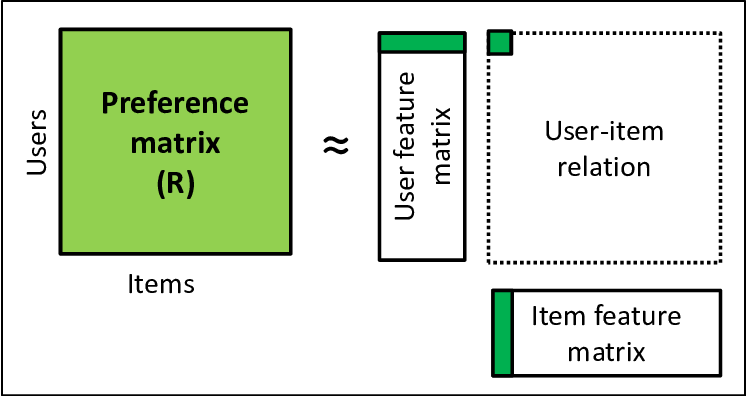
\includegraphics[width=1\linewidth]{matrix-factorization}}
					\end{minipage}
				\end{figure}
			Algorithms: Alternating least squares(ALS), Stochastic gradient descent(SGD) 
		\end{frame}
		
		\begin{frame}
			\frametitle{Matrix-factorization}
			\begin{figure}[h]
				\begin{minipage}[h]{0.75\linewidth}
					\center{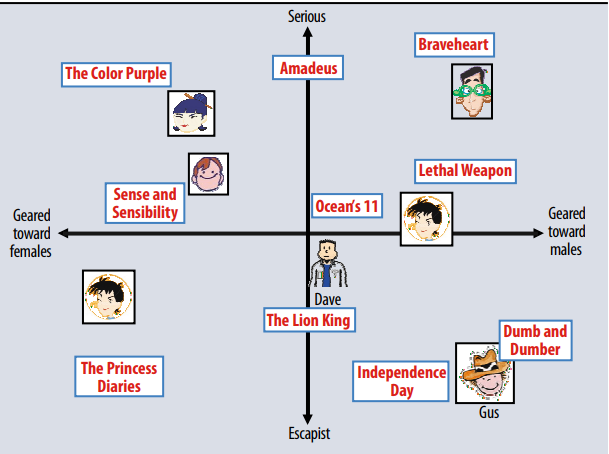
\includegraphics[width=1\linewidth]{features_space}}
				\end{minipage}
			\end{figure}
		\end{frame}
		
		\begin{frame}
			\frametitle{Photon-ml}
			\begin{figure}[h]
				\begin{minipage}[h]{1.1\linewidth}
					\center{
\includegraphics[width=1\linewidth]{linkedin}}
				\end{minipage}
			\end{figure}
		\end{frame}
		
		\begin{frame}
			\frametitle{Photon-ml}
			\begin{itemize}
				\item Generalized Linear Model (GLM)
				\item Generalized Additive Model (GAM)
				\item Generalized Additive Mixed-Effect Model(GAME)
				\item GLMix(Generalized Linear Mixed) = GLM + per-user model + per-item model
			\end{itemize}
		\end{frame}
		
		
		\begin{frame}
			\frametitle{Photon-ml}
			\begin{figure}[h]
				\begin{minipage}[h]{1.1\linewidth}
					\center{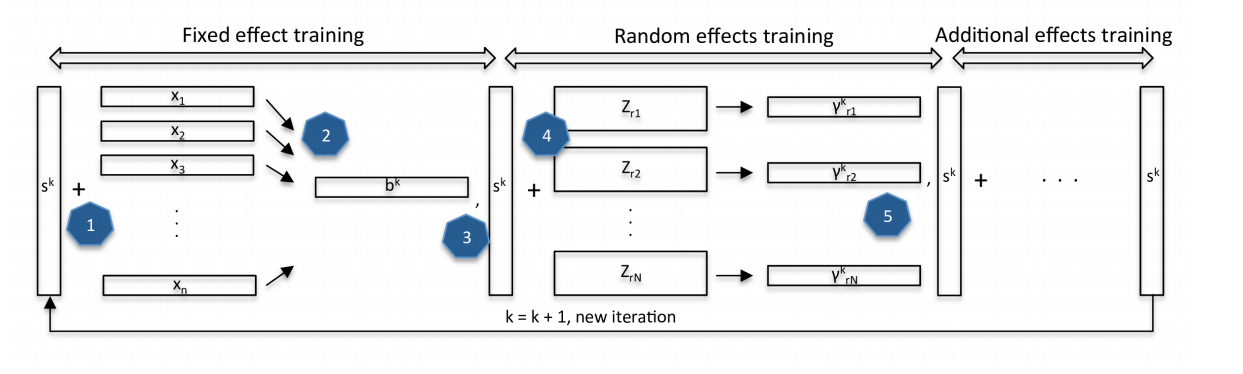
\includegraphics[width=1\linewidth]{pipline_photon}}
				\end{minipage}
			\end{figure}
			The experiments were conducted on a cluster consisting of 135 nodes managed by Apache YARN 3. Each node has 24 Intel Xeon(R) CPU E5-2640 processors with 6 cores at
			2.50GHz each, and every node has 250GB memory.
		\end{frame}
		
		\begin{frame}
			\frametitle{Evaluation}
			\begin{figure}[h]
				\begin{minipage}[h]{1.1\linewidth}
					\center{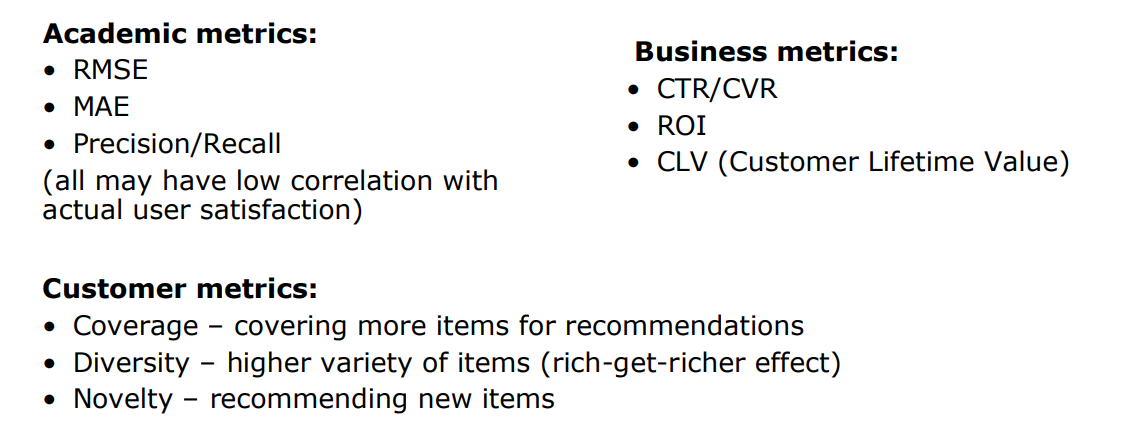
\includegraphics[width=1\linewidth]{evaluation}}
				\end{minipage}
			\end{figure}
		\end{frame}
				
		\begin{frame}
			\frametitle{Проблемы}
			\begin{itemize}
				\item Товары быстро продаются, не успев даже набрать хорошую историю по просмотрам и запросам контактов. Классические алгоритмы коллаборативной фильтрации устроены так, что объявления с короткой историей не попадают в рекомендации. Чаще рекомендуются долго живущие объявления, которые, как правило, представляют меньший интерес для покупателей.
				\item Проблемы холодного старта
				\item Как заставить это все быстро работать
			\end{itemize}
		\end{frame}

		\begin{frame}
		\frametitle{Проблемы}
				\begin{figure}[h]
					\begin{minipage}[h]{0.2\linewidth}
						\center{
\includegraphics[width=1\linewidth]{spark}}
					\end{minipage}
					\begin{minipage}[h]{0.3\linewidth}
						\center{
\includegraphics[width=1\linewidth]{hadoop}}
					\end{minipage} \\
					\begin{minipage}[h]{0.2\linewidth}
						\center{
\includegraphics[width=1\linewidth]{hive}}
					\end{minipage}
					\begin{minipage}[h]{0.2\linewidth}
						\center{
\includegraphics[width=1\linewidth]{elastic}}
					\end{minipage}
				\end{figure}
		\end{frame}

		\begin{frame}
			\begin{center}
				Спасибо за внимание!
			\end{center}
		\end{frame}
		
	\end{document} 